\subsection{Bluez : Userspace}
\begin{frame}
\begin{minipage}[t]{0.60\linewidth}
	\begin{figure}
		\includegraphics[height=5cm]{bluetoothd.png}
		\caption{bluetoothd}
	\end{figure}
\end{minipage}
\begin{minipage}[t]{0.30\linewidth}
	\begin{block}{Démon bluetoothd}
		\begin{itemize}
			\item Uniformisation
			\item Abstraction
		\end{itemize}
		Commandes : 
		\begin{itemize}
			\item Données
			\item Configuration
			\item Évènements
		\end{itemize}
	\end{block}
\end{minipage}
\end{frame}

\begin{frame}
\begin{minipage}[t]{0.60\linewidth}
	\begin{figure}
		\includegraphics[height=5cm]{bluetoothd.png}
		\caption{Profils Externes}
	\end{figure}
\end{minipage}
\begin{minipage}[t]{0.30\linewidth}
	\begin{block}{oFono}
		\begin{itemize}
			\item Uniformisation
			\item Abstraction
		\end{itemize}
	\end{block}
	\begin{block}{connman}
		\begin{itemize}
			\item Uniformisation
			\item Abstraction
		\end{itemize}
	\end{block}
	\begin{block}{pulse audio}
		\begin{itemize}
			\item Uniformisation
			\item Abstraction
		\end{itemize}
	\end{block}
\end{minipage}
\end{frame}

\begin{frame}
ofono connman pulseaudio
\end{frame}

\begin{frame}
hcitool hciconfig hci* btmon
\end{frame}

\begin{frame}
btgatt-client + example*
\end{frame}

\begin{frame}
API
\end{frame}


